\subsection{Bestimmung der Verdampfungswärme bei kleinem Druck}
\label{sec:bestimmungverdampfungswarme}
Die Verdampfungswärme kann -- aus dem idealen Gasgegesetz \eqref{ideales Gas} abgeleitet --  als Porportionalitätsfaktor zwischen dem natürlichen Logarithmus des Druckes $P$ und der reziproken absoluten Temperatur $T$ aufgefasst werden. 
\begin{equation}
\ln(P) = - \frac{L}{\text{R}} \frac{1}{T} + \text{const.} = a \cdot \frac{1}{T} +b
\end{equation}



Die Wertepaare sind in Tabelle \ref{tab:druck-temperatur} dargestellt.
\begin{figure}[h!]
\captionof{table}{Wertepaare für die lineare Regression}	
	\centering
\begin{tabular}{c|c}
	Reziproke absolute Temperatur in \si{\kelvin}&   Logarithmus des Druckes ($\ln{(P/P_0)}$) \\
	\hline
	0.003095 &                   9.532 \\
	0.003047 &                   9.687 \\
	0.003002 &                   9.903 \\
	0.002957&                  10.142  \\
	0.002914 &                  10.342 \\
	0.002872 &                  10.551  \\
	0.002831 &                  10.773 \\
	0.002792 &                  10.979  \\
	0.002753 &                  11.155  \\
	0.002716 &                  11.327 \\
	0.002680&                  11.523 \\
\end{tabular}
\label{tab:druck-temperatur}
\end{figure}


Lineare Regression nach Formeln aus Kapitel (\ref{sec:regression}) mittels Python liefert
\begin{equation}
a= \num{-4910(60)} \, \si{\kelvin}
\end{equation}
und damit eine Verdampfungswärme des Wassers von
\begin{equation}
L = - a \cdot R = \SI{40800(500)}{\joule\per\mol} 
\end{equation}
wobei $R$ die Gaskonstante mit \SI{8.314}{\joule\per\kelvin\per\mol} ist. \\
.


\begin{figure}[h!]
	\centering
	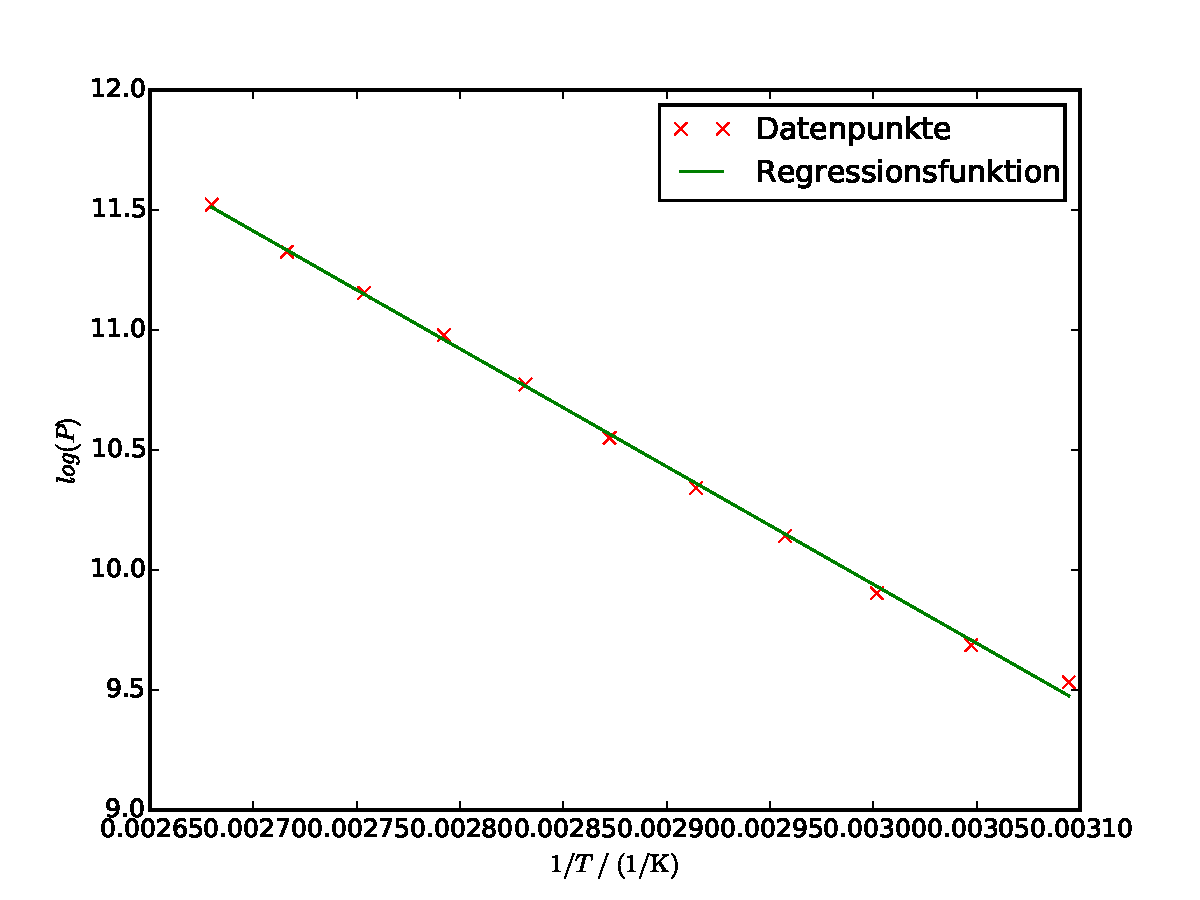
\includegraphics[width=0.95\textwidth]{L_kleiner_Druck.pdf}
	\caption{Logarithmus des Dampfdruckes gegen die reziproke absolute Temperatur}
	\label{fig:L_kleiner_Druck}
\end{figure}

\subsection{Unterscheidung zwischen äußerer und innerer Verdampfungswärme}
Die äußere Verdampfungswärme entspricht der Energie, die von System aufgewendet wird um zu expandieren. Diese Volumenarbeit ist bei einer Temperatur von  \SI{373}{\kelvin}
\begin{equation}
L_\text{a} = p \cdot V_\text{m} = R \cdot T = \SI{8.314}{\joule\per\kelvin\per\mol} \cdot  \SI{373}{\kelvin} \approx \SI{3101}{\joule\per\mol} \quad.
\end{equation}
Die innere Verdampfungswärme wird aufgebracht, um die wechselwirkenden Moleküle voneinander zu trennen. Da in Abschnitt \ref{sec:bestimmungverdampfungswarme} die gesamte Verdampfungswärme bestimmt wurde, entspricht die innere Verdampfungswärme gerade
\begin{align}
L_\text{i} &= L - L_{\text{a}} = \SI{40800}{\joule\per\mol} - \SI{3101}{\joule\per\mol} = \SI{37699}{\joule\per\mol} \\
&\widehat{=} \SI{2.353e23}{\eV\per\mol} \widehat{=} \ 0.391 \, \frac{\si{\eV}}{\text{Molukül}}\quad.
\end{align}





\subsection{Temperaturabhängigkeit der Verdampfungswärme bei hohem Druck}
Die Druck- und Temperaturabhängigkeit der Verdampfungswärme ist nach Formel \eqref{Clausius einfach} mit
\begin{equation}
	L(T, p(T)) = T^2\frac{R}{p}\frac{\text{d}p}{\text{d}T}
\end{equation} gegeben.

Zunächst wird der Druck als Funktion der Temperatur dargestellt. Mit Hilfe von Python wurde für $p(T)$ ein Polynom dritten Grades berechnet. Die hier angegebenen Werte für die Koeffizienten des Polynoms sind gerundet, obwohl mit exakten weiter gerechnet wurde.
\begin{equation}
p(T) = a \cdot T ^3 + b \cdot T^2 +c \cdot T + d
\end{equation}
\begin{align}
a &=\SI{0.63(33)}{\pascal\per\kelvin\cubed}  \\
b &= \SI[per-mode = fraction]{640(370)}{\pascal\per\kelvin\squared}  \\
c &= \SI{221000(146000)}{\pascal\per\kelvin} \\
d  &= \SI{25800000(1870000)}{\pascal}
\end{align}


Die Ableitung des Druckes nach der Zeit ist
\begin{equation}
\frac{\text{d} p}{\text{d} T} = 3 \cdot a \cdot T^2 + 2 \cdot b \cdot T + c
\end{equation}
\begin{figure}[h!]
	\centering
	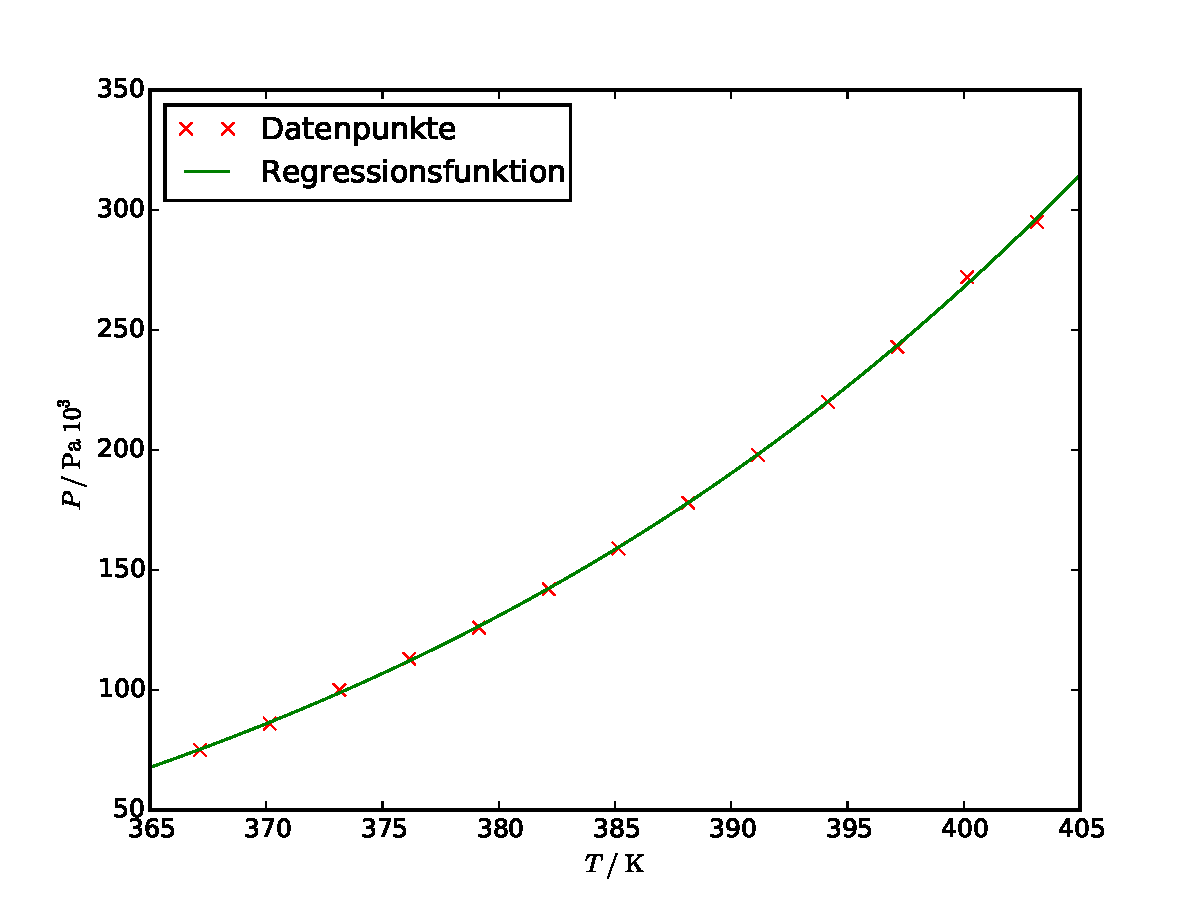
\includegraphics[width=0.95\textwidth]{Regerssionspolynom_P(t).pdf}
	\caption{Regressionspolynom dritten Grades des Druckes über der Temperatur}
	\label{fig:Regerssionspolynom_P(t)}
\end{figure}
\\

Die Volumenabhängigkeit von Temperatur und Druck kann hier nicht mehr vernachlässigt werden. Das ideale Gasgesetz gilt nicht, sodass das Molvolumen besser durch
\begin{equation}
\left( p(T) + \frac{a_\text{W}}{V_\text{m}^2}\right) = R \cdot T
\end{equation}
\begin{equation}
\Leftrightarrow
V_{m,+,-}(T, p(T)) = \frac{R \cdot T \pm \sqrt{R^2 \cdot T^2 - 4 \cdot a_\text{W} \cdot p(T)}}{2 \cdot p(T)}
\end{equation}
genähert wird. Wobei $a_\text{W}$ eine stoffspezifische Konstante ist
\begin{equation}
a_\text{W} = \SI{0.9}{\joule\metre^3\per\mol^2} \quad.
\end{equation}

 Nach Einsetzen der Ergebnisse und Betrachtung der Abbildung \ref{fig:volumen} ist ersichtlich, dass die Lösung $V_{m,+}$ das reale Volumen wiedergibt, da Wasser nach der idealen Gasgleichung unter Normalbedingungen ein Molvolumen von \SI{22.7}{\liter\per\mol} hat.
\begin{figure} 
	\centering
	\begin{subfigure}{\textwidth}
		\centering
		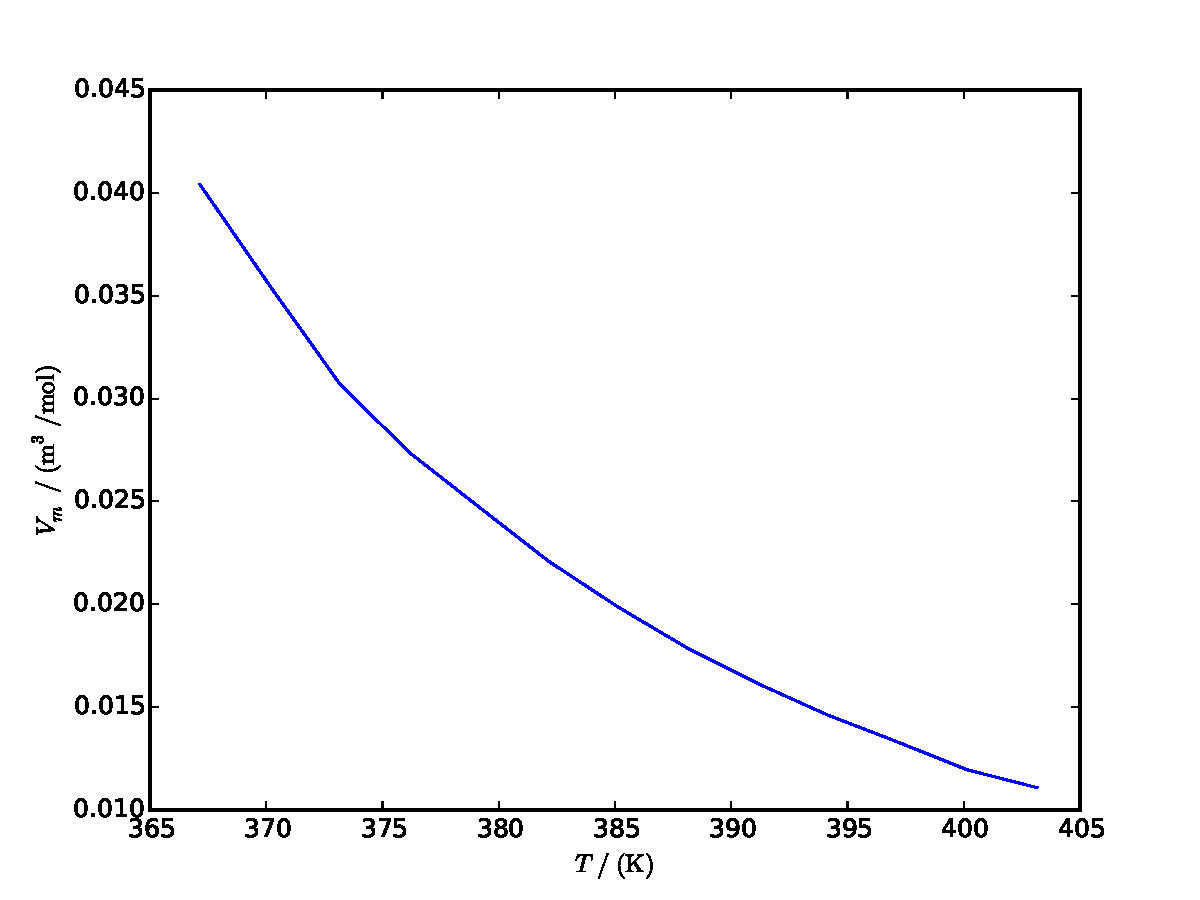
\includegraphics[width=\textwidth]{Volumen+.pdf}
		\caption{Volumen, plus}
	\end{subfigure}
	\begin{subfigure}{\textwidth}
		\centering
		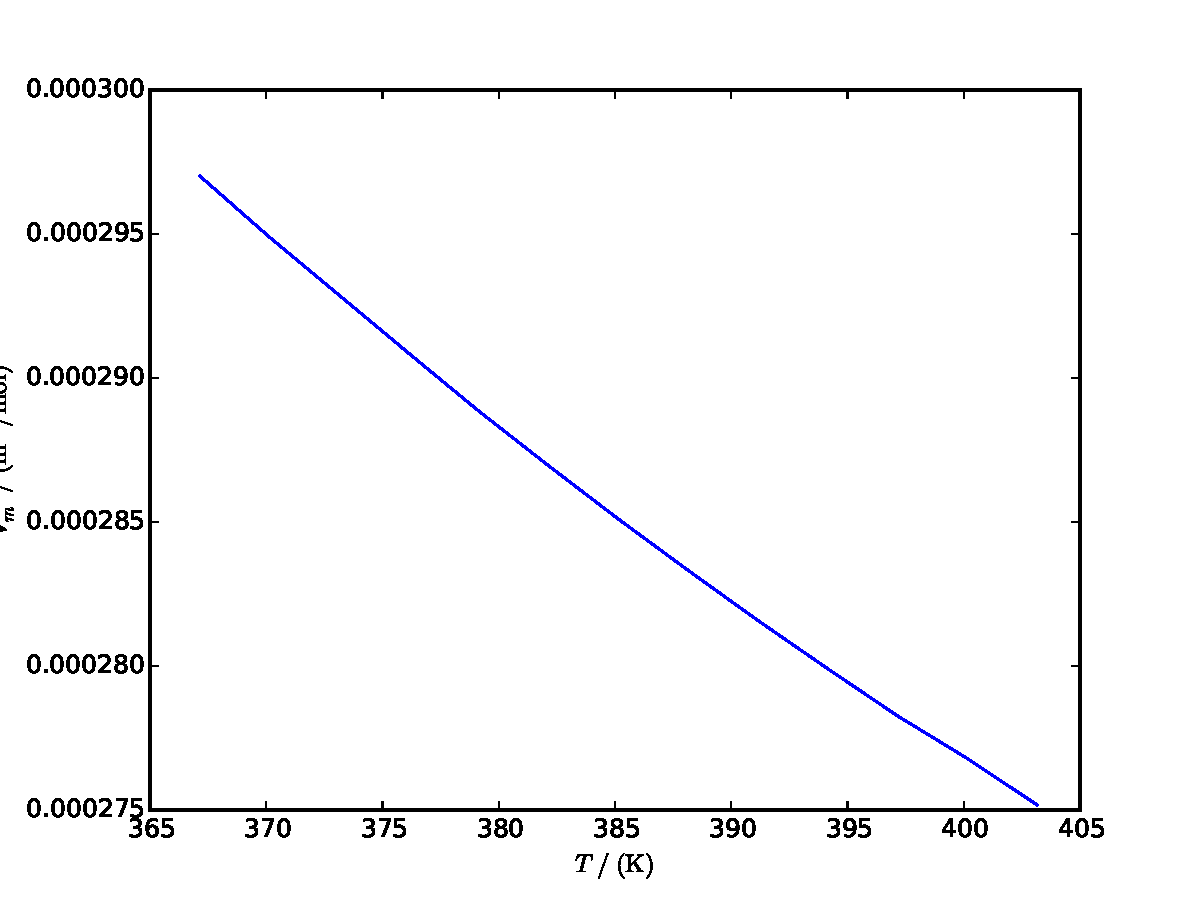
\includegraphics[width=\textwidth]{Volumen-.pdf}
		\caption{Volumen, minus}
	\end{subfigure}
	\caption{Volumina mit der positiven und negativen Wurzel }
	\label{fig:volumen}
\end{figure}


Nach dieser Vorarbeit ist
\begin{align}
& L(T, p(T)) = V_{m,+}(T, p(T)) \cdot T \cdot \frac{\text{d} p}{\text{d} T} \\
&= \left(\frac{R \cdot T + \sqrt{R^2 \cdot T^2 - 4 \cdot a_\text{W} \cdot p(T)}}{2 \cdot p(T)}\right)  \cdot T \cdot \left(3 \cdot a \cdot T^2 + 2 \cdot b \cdot T + c \right) %\\
%=\left(\frac{R \cdot T + \sqrt{R^2 \cdot T^2 - 4 \cdot a_\text{W} \cdot (a \cdot T ^3 + b \cdot T^2 +c \cdot T + d)}{2 \cdot (a \cdot T ^3 + b \cdot T^2 +c \cdot T + d)}\right)  \cdot T \cdot \left(3 \cdot a \cdot T^2 + 2 \cdot b \cdot T + c \right)
\end{align}

und wurde in Abbildung \ref{fig:L_groser_druck_temperaturabhangig} über die Temperatur aufgetragen. Zusätzlich wurden die Werte eingetragen, die sich ergeben, wenn die Messwerte von $T$ in $L(T, p(T))$ eingesetzt werden. Die Datenpunkte sind die $L(T_\text{gemessen})$ und zusätzlich in Tabelle \ref{tab:verdampfungswarme} dargestellt. 
\begin{figure}[h!]
	\captionof{table}{Temperaturabhängige Verdampfungswärme}	
	\centering
\begin{tabular}{c|c}
	Temperatur in $\si{\kelvin}$ &   Verdampfungswärme in $\si{\joule\per\mol}$ \\
	\hline
	367.15 &                                      53560.1 \\
	370.15 &                                      51431.8 \\
	373.15 &                                      48777.2 \\
	376.15 &                                      47649.1 \\
	379.15 &                                      47178.4 \\
	382.15 &                                      46184.9 \\
	385.15 &                                      45462.1 \\
	388.15 &                                      44697.8 \\
	391.15 &                                      44160.9 \\
	394.15 &                                      43601.7 \\
	397.15 &                                      43227.3 \\
	400.15 &                                      42192.1 \\
	403.15 &                                      42447.3 \\
\end{tabular}
	\label{tab:verdampfungswarme}
\end{figure}





\begin{figure}[h!]
	\centering
	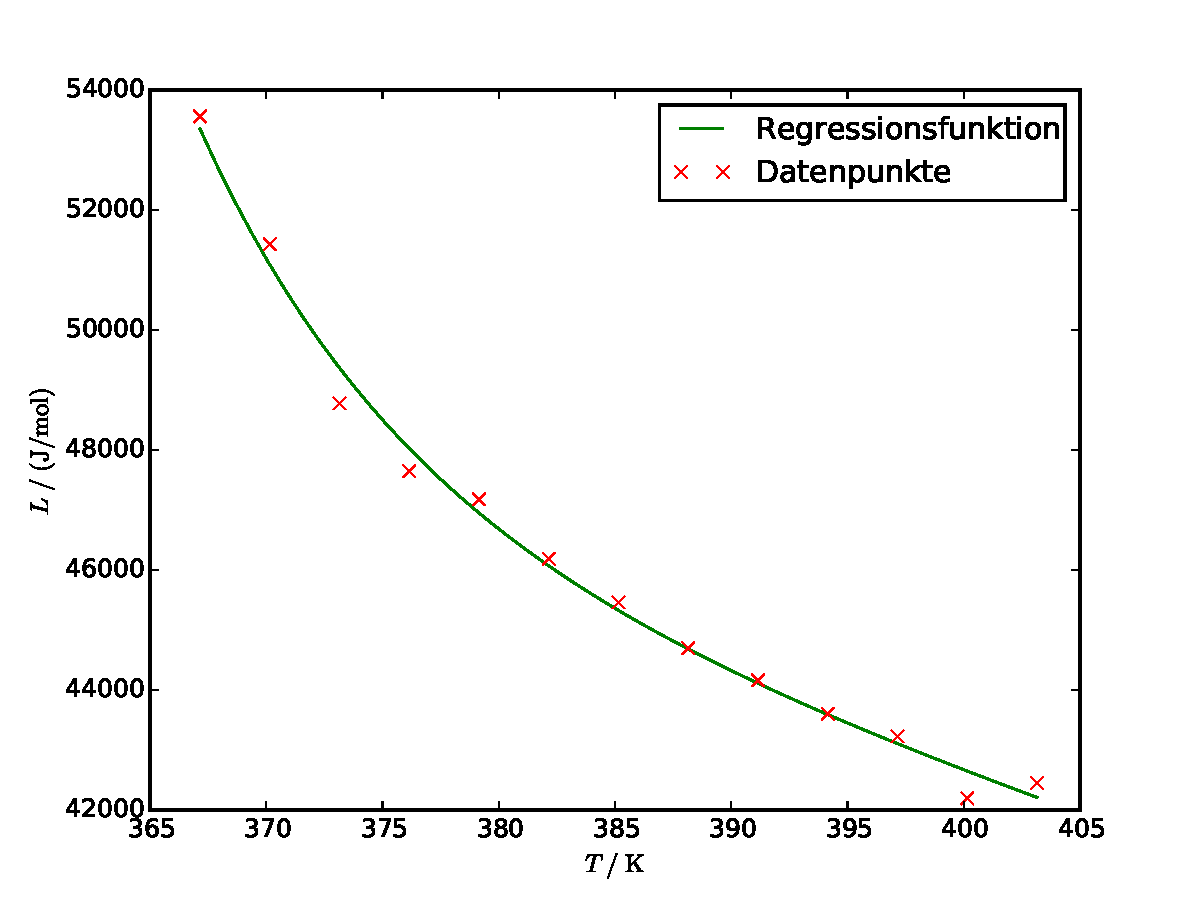
\includegraphics[width=0.95\textwidth]{L_groser_druck_temperaturabhangig.pdf}
	\caption{Verdampfungswärme in Abhängigkeit der Temperatur}
	\label{fig:L_groser_druck_temperaturabhangig}
\end{figure}





